\begin{figure}[!ht]
	\centering
	\setlength{\resLen}{6.25in}
	\setlength{\raiseLen}{0.35in}
	\addtolength{\tabcolsep}{-4pt}
	\begin{tabular}{cc}
		\raisebox{0.5\raiseLen}{\rotatebox[origin=c]{90}{\small Input}} &
		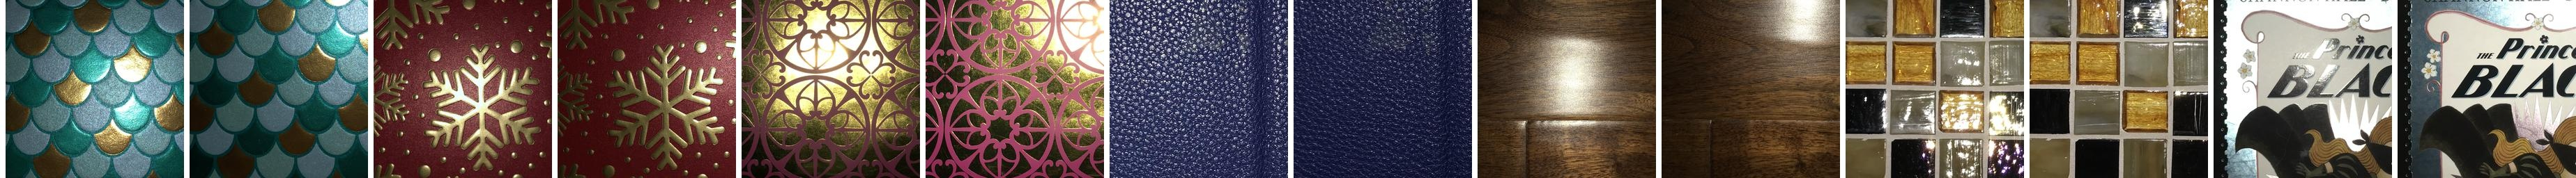
\includegraphics[width=\resLen]{svbrdf/teaser/refs.jpg}
		\\[-2pt]
		\raisebox{\raiseLen}{\rotatebox[origin=c]{90}{\small Rendering}} &
		\animategraphics[width=\resLen,loop,alttext=]{5}{svbrdf/teaser/teaser_}{001}{024}
		\\[-2pt]
		\raisebox{\raiseLen}{\rotatebox[origin=c]{90}{\small Est. maps}} &
		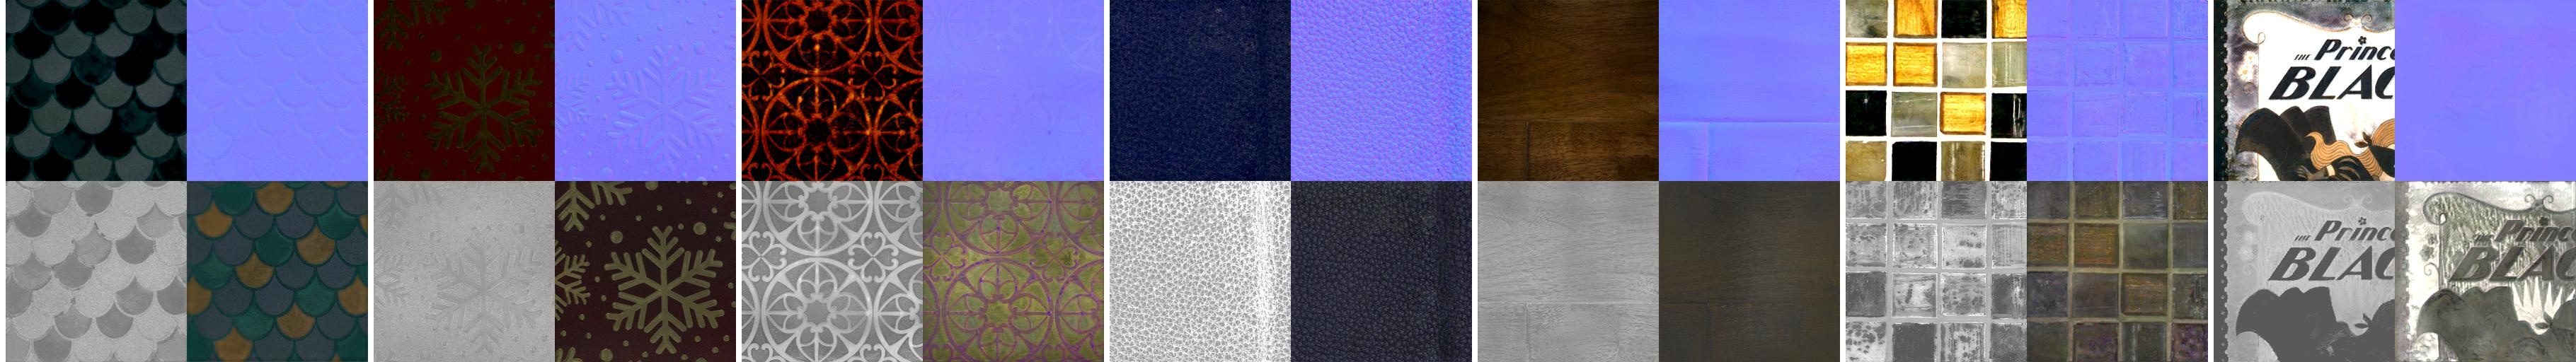
\includegraphics[width=\resLen]{svbrdf/teaser/maps.jpg}
	\end{tabular}
	\caption[Teaser]{\label{fig:svbrdf:teaser}
		We introduce a method to capture SVBRDF material maps from a small number of mobile flash photographs, achieving high quality results both on original and novel views. Our key innovation is optimization in the latent space of MaterialGAN, a generative model trained to produce plausible material maps; MaterialGAN thus serves as a powerful implicit prior for result realism. Here we show re-rendered views for several different materials under environment illumination. We use 7 inputs for these results (with 2 of them shown).
		(Please use Adobe Acrobat and click the renderings to see them animated.)
	}
\end{figure}
